\chapter{Concluding Remarks and Future Research}
We have presented a method to quadrangulate a triangle-mesh interactively by solving a smooth unconstrained optimization problem, and designed a tool to demonstrate it in action. Our method produce decent preliminary results, but yet to be sufficient for extracting a quad mesh. As can be seen in chapter \ref{chapter:results}, the Cartesian grid isolines do form a valid quad mesh over the 3D surface of the presented models, but failures can be spotted where the isolines are discontinues. Figure \ref{fig:failues} demonstrate surface areas where our method failed to satisfy the integer-grid maps conditions.
\begin{figure}[ht]
\centering
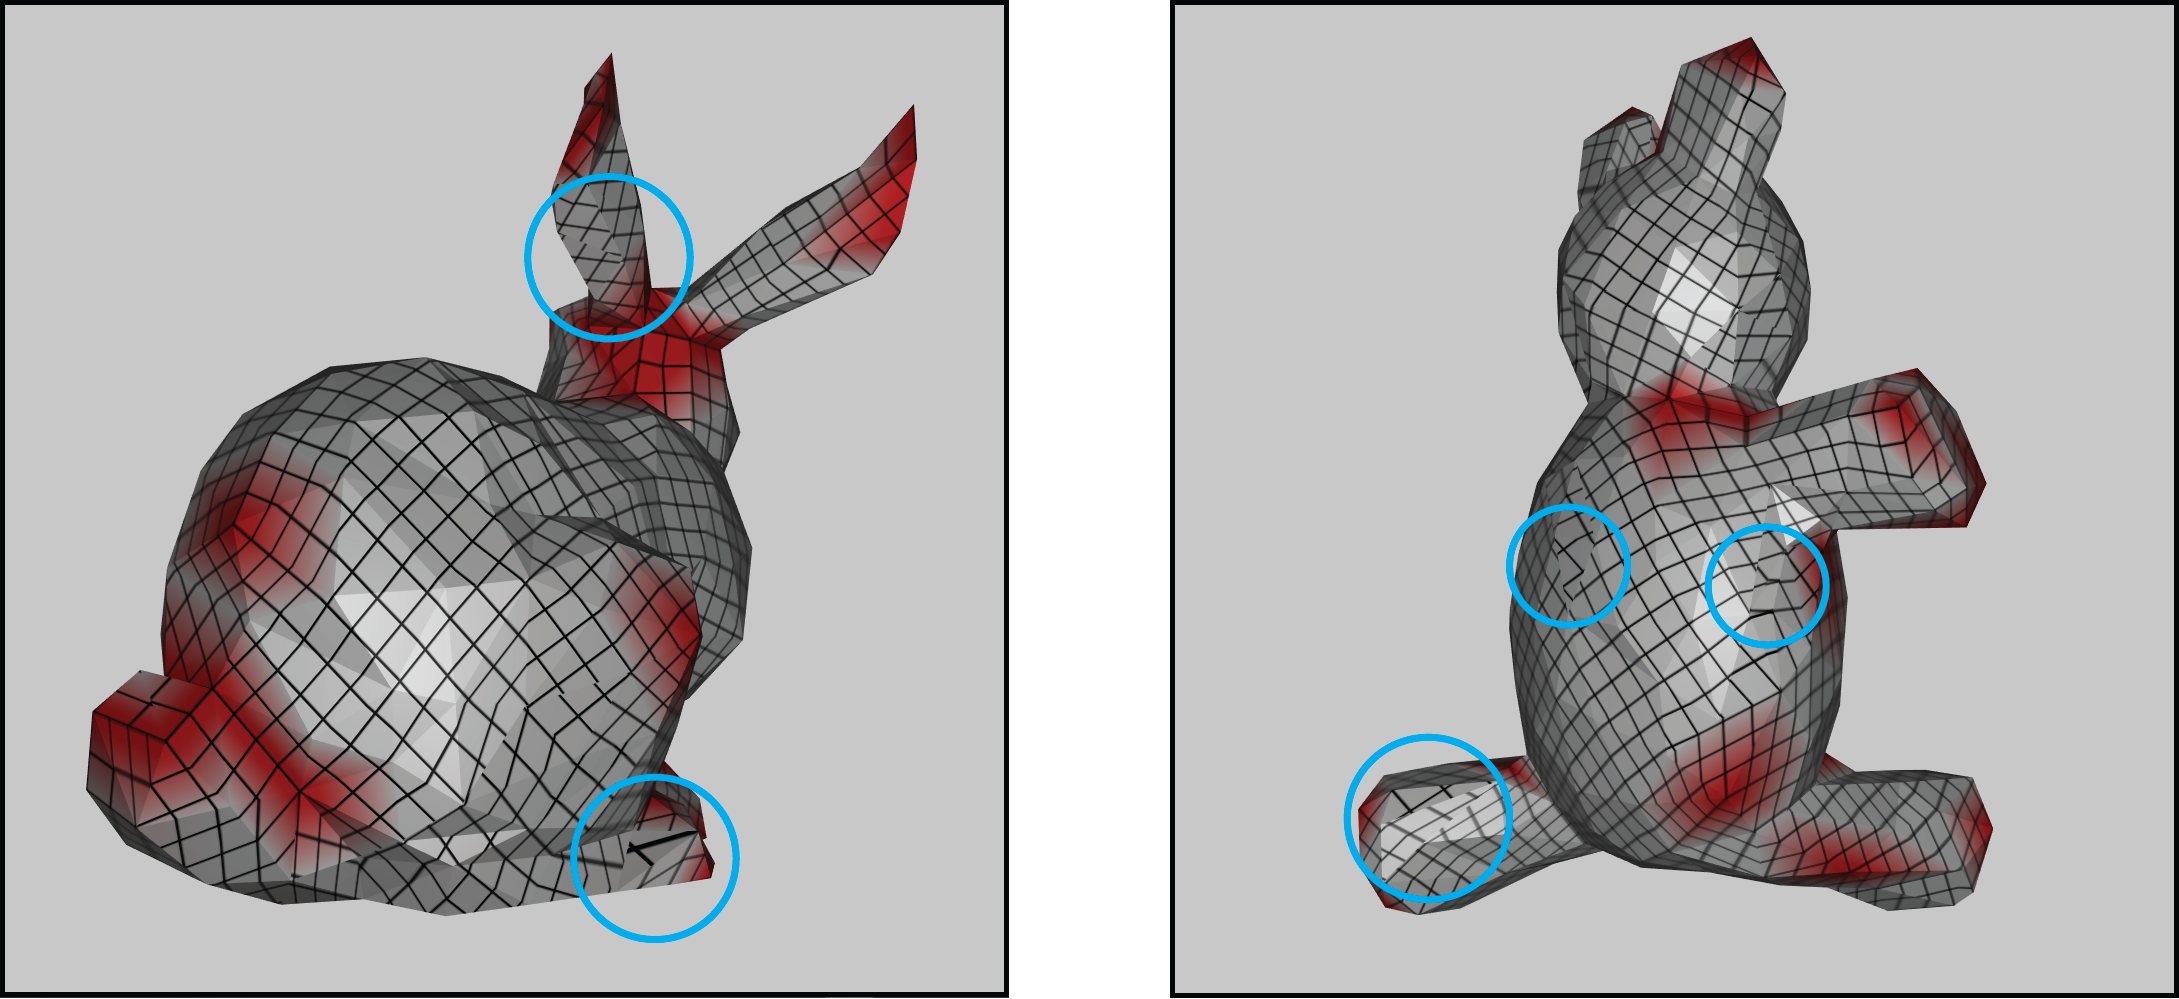
\includegraphics[width=13cm]{figures/results/failures.png}
\caption[Failure Spots of Our Method]{The blue circles mark areas on the surfaces where the continuity of the Cartesian isolines breaks}
\label{fig:failues}
\end{figure}

\noindent We believe our method can be further improved, both by means of its penalty functions formulation and by its graphic user interface. We present numerous ideas for future research work:
\paragraph{Unified Penalty Function for Angle and Length}
The separation between the angle and length penalty functions is technical and artificial, it makes it harder for the end-user to control the optimization process, and it introduce unnecessary inconsistent sensitivity for weight perturbations. We propose to use instead the following penalty function for two half-edges $e_i$ and $e_j$:
\begin{flalign}
P_{unified} = \norm{R\left(e_i, e_j\right)^4 - I}_F^2
\end{flalign}
Where $R\left(e_i, e_j\right)$ is the linear transformation induced by the two coordinate system defined by $e_i$ and $e_j$, when treated as vector sharing the same origin. Figure \ref{fig:unified} the two coordinate systems that defines $R\left(e_i, e_j\right)$. If $R\left(e_i, e_j\right)^4$ equals the identity matrix, then the two half-edges must have the same length be an integer multiple of $90^\circ$ degrees apart.
\begin{figure}[ht]
\centering
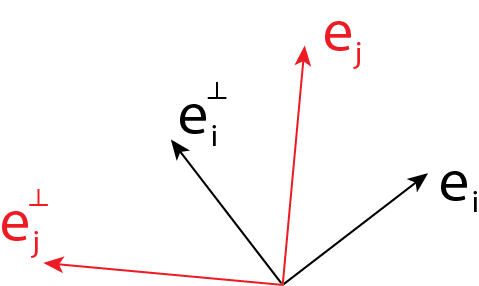
\includegraphics[width=8cm]{figures/unified_energy.png}
\caption[Unified Energy Coordinate Systems]{$R\left(e_i, e_j\right)$ is the linear transformation that takes the black vector onto their corresponding red vectors.}
\label{fig:unified}
\end{figure}
\paragraph{Orientation Field}
We believe that we can achieve superior results by aligning the partial derivative vectors of the parametrization mapping with the principal curvature directions, or any other given orientation field, such as brush strokes painted by the user. To achieve it, one can formulate an additional penalty function, as described in \cite{10.1145/1531326.1531383}.
\paragraph{Manual Location of Singular-Points}
We believe that the user can have a great benefit from being able to manually select where singular-points will be located. To achieve it, it is possible to define an additional penalty function, which will penalize set of twin-vertices for having \textbf{zero} angular defect.
\paragraph{Modified Piece-wise Polynomial Periodic Function}
The piece-wise polynomial periodic function, as defined in appendix \ref{appendix:a}, has an unnecessary wide non-convex region around its peak points. One can redefine it to have a narrower non-convex region, with the price of widening the local minimum plateaus. It might help to eliminate saddle points on the main objective function, at the price of longer convergence time.